\documentclass[10pt]{article}
\usepackage[total={170mm,230mm}]{geometry}

\usepackage{cmap}
\usepackage[utf8]{inputenc}
\usepackage[T2A]{fontenc}
\usepackage[russian]{babel}
\usepackage{hyphsubst}

\usepackage{graphicx}
\usepackage{xcolor}
\usepackage{amssymb}
\usepackage{amsfonts}
\usepackage{amsmath}
\usepackage{amsthm}
\usepackage{physics}
\usepackage{wrapfig}
\usepackage{cancel}
\usepackage{pdfpages}
\usepackage{hyperref}
\usepackage{caption}
\usepackage{subcaption}
% \usepackage{bibtex}

\title{Домашнее задание №7. Решение эволюционной задачи в скалированных координатах}
\author{Александр Козлов}
\date{\today}

\begin{document}

\maketitle

\section*{Формулировка задания}

Рассматривается временное уравение Шрёдингера (УШ) $i\partial_t \Psi = \mathrm{H} \Psi$ с начальным условием $\Psi(k,t=0) = \exp(-(k-k_0)^2)$, где $k$ --- волновое число (в атомных единицах --- в которых мы работаем --- тождественно импульсу). Необходимо воспроизвести свбодную (то есть $\mathrm{H}=-\laplacian$ в атомарных единицах) динамику гауссовского волнового пакета с использованием скалированных координат.

\section{Аналитическое решение}

В начальный момент времени $t=0$ волновая функция в импульсном пространстве имеет вид $$\Psi(k,t=0) = \exp(-(k-k_0)^2),$$ где $k$ --- волновое число (в атомных единицах --- в которых мы работаем --- тождественно импульсу). Гамильтониан свободного пространства в импульсном пространстве имеет вид $$ \mathrm{H} = k^2,$$ поэтому решение времянного УШ в импульсном пространстве легко написать. Оно будет иметь вид:
\begin{equation}
 \Psi(k,t) =\exp\qty(-i k^2 t - (k-k_0)^2).
\end{equation}
В прострвенных координатах $x$ такая волновая функция будет иметь вид:
\begin{equation}
 \Psi(x,t) =  C \cdot \int \dd{k} \exp\qty(ikx -i k^2 t - (k-k_0)^2) = C \cdot \sqrt{\dfrac{\pi}{it+1}} \exp\qty(\dfrac{(2k_0 + ix)^2}{4(it+1)} - k_0^2),
\end{equation}
где $C$ --- некоторый нормировочный множитель. Выберем $C$ таким образом, чтобы $\norm{\Psi(x,t=0)}^2=1$. Тогда $C=(2\pi^3)^{-1/4}$ и аналитическое решение имеет вид:
\begin{equation}
 \Psi(x,t) = \sqrt[4]{\dfrac{1}{2\pi}} \sqrt{\dfrac{1}{it+1}} \exp\qty(\dfrac{(2k_0 + ix)^2}{4(it+1)} - k_0^2).
\end{equation}

\section{Решение эколюционной задачи в скалированных координатах}

Исходное одномерное УШ имеет вид $i\partial_t \Psi(x,t) = -\partial_{xx} \Psi(x,t)$. Делаем замену переменных $x = R(t) \xi$ и переходим к уравнению
\begin{equation}
 i\partial_t \Phi = \mathrm{H}_\xi\Phi, \quad \mathrm{H}_\xi = -\dfrac{1}{R^2} \partial_{\xi\xi} + \dfrac{1}{4}R(t)\ddot{R}(t)\xi^2
\end{equation}
на волновую функцию $\Phi(\xi,t)$, связанную с волновой функцией исходной задачи соотношением
\begin{equation}
 \Psi(x,t) = \dfrac{1}{\sqrt{R}} \exp\qty[-\dfrac{i}{4} \dot{R}(t) R(t) \xi^2(x,t) ] \Phi(\xi(x,t),t).
\end{equation}
Видно, что уравнение на новую волновую функцию эквивалентно УШ с времязависящим гамильтанианом. Эволюционную задачу будем решать, используя следующую  аппроксимацию оператора эволюции:
\begin{equation}
 U(t_2,t_1) = \exp\qty[-i\int_{t_1}^{t_2} \mathrm{H}_\xi \dd{t}]\approx\exp\qty[-i\; \mathrm{H}_\xi\qty(\frac{t_1+t_2}{2})\cdot (t_2 - t_1)].
\end{equation}


\section{Результаты и сопоставление численного решения с аналитическим}

\begin{figure}[htbp]
 \centering
 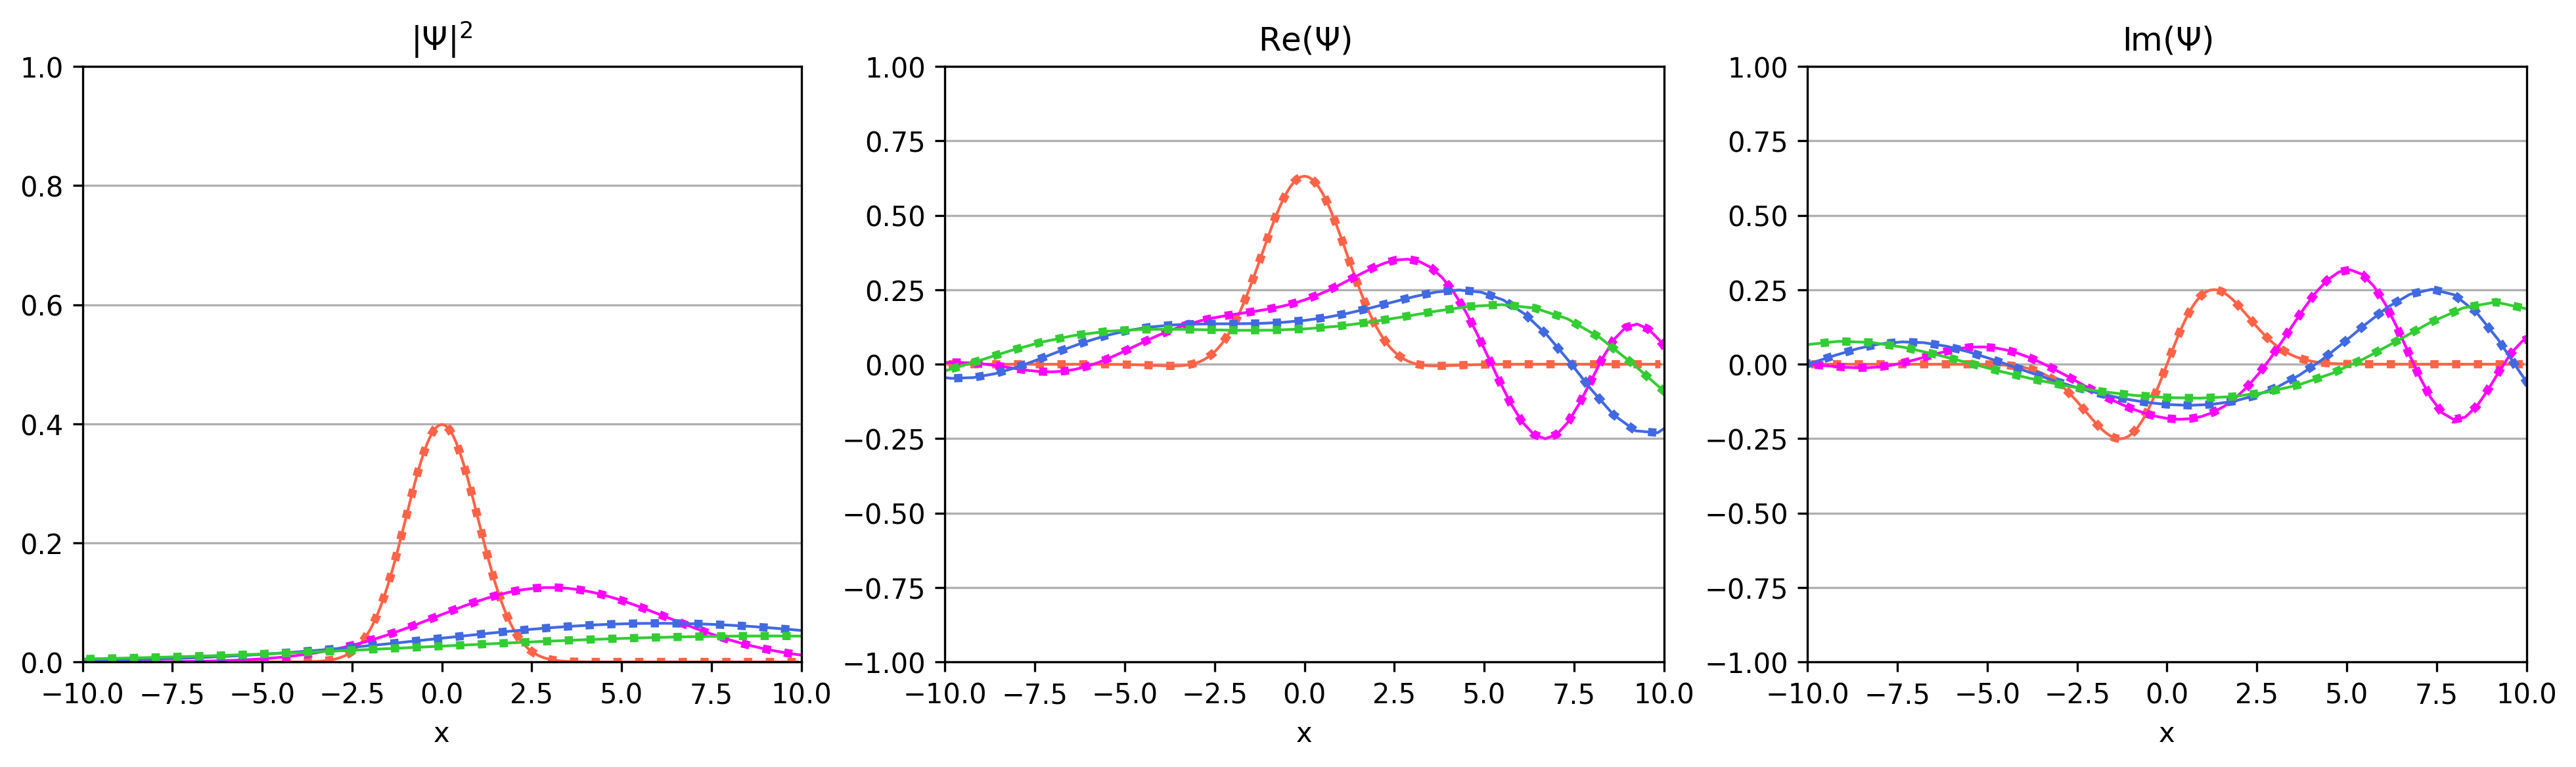
\includegraphics[width=\textwidth]{../figures/comparison.png}
 \caption{Сравнение численного и аналитических решений. Точки соответсвуют численному решению, а непрервная линия --- аналитическому. Красный цвет обозначает волновые функции при $t=0$, маджента~---~при $t=0.3$, королевский голубой --- при $t=0.6$ и лаймовый зеленый~---~при $t=0.9$. Шаг по времени $\Delta t = 0.1$, а импульс волновой функции $k_0 = 0.5$.}
 \label{fig:1}
\end{figure}






\end{document}
